\subsection[Ozone as a Function of NOx and Temperature]{Ozone as a Function of \ce{NO_x} and Temperature} \label{ss:r_contours} 
\begin{figure}%
    \centering%
    \caption{Contours of maximum ozone mixing ratios (ppbv) as a function of the total \ce{NO_x} emissions on the first day and temperature for each chemical mechanism using a temperature-dependent and temperature-independent source of isoprene emissions.}
    \label{f:ozone_contours}%
    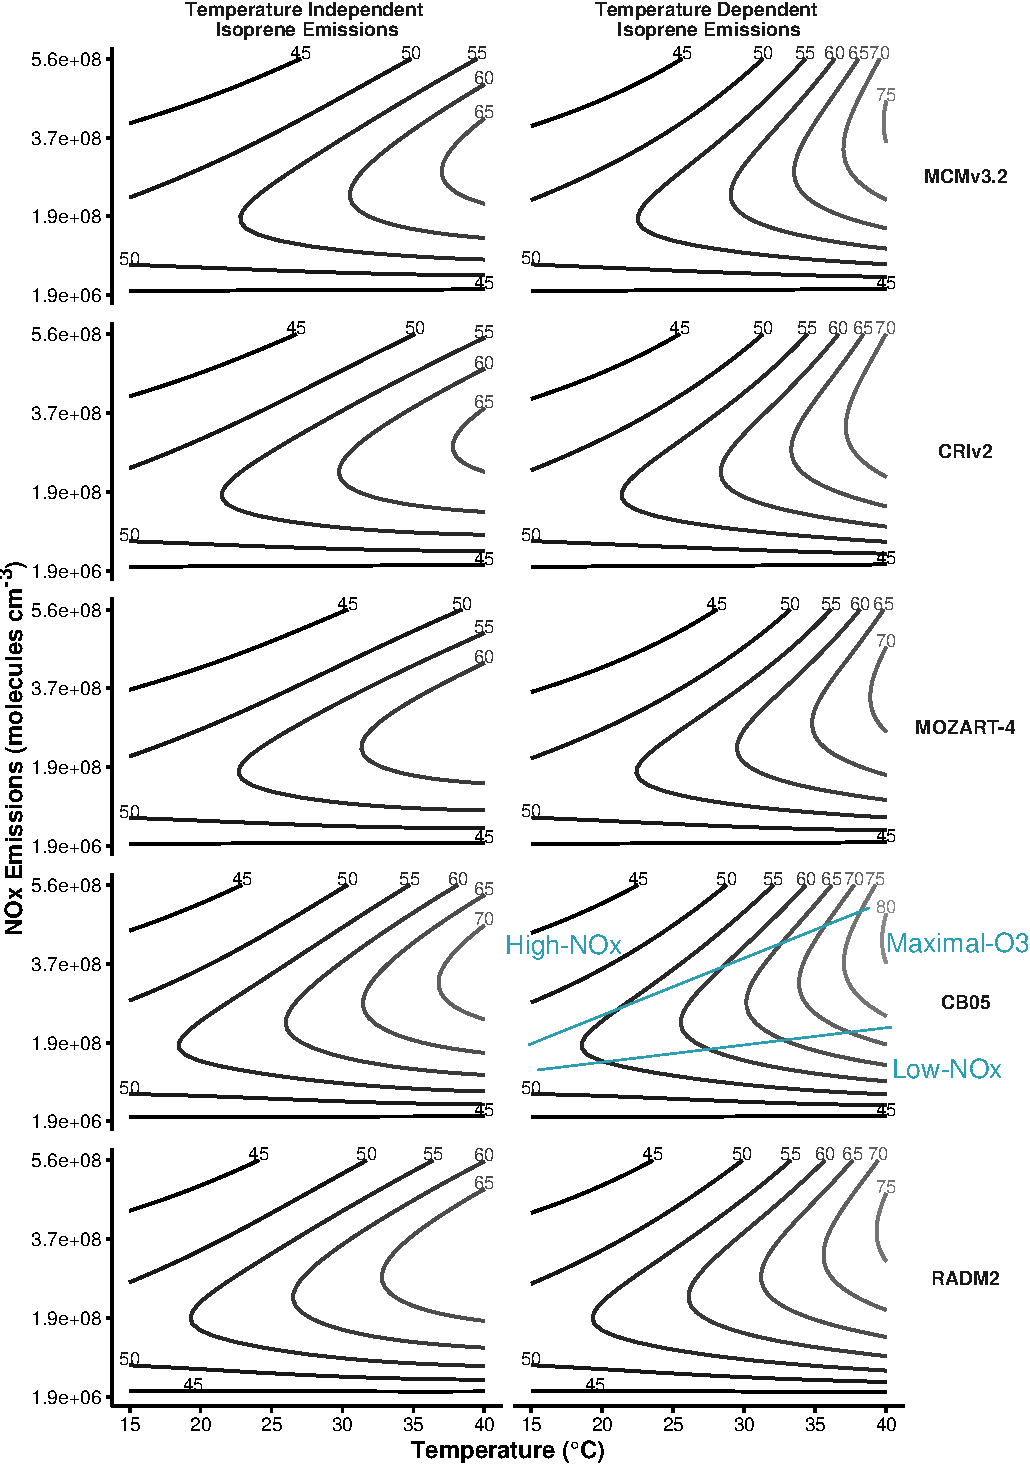
\includegraphics[width=\textwidth]{img/O3_comparison}%
\end{figure}

\begin{figure}[t]%
    \centering%
    \caption{Ozone mixing ratios (ppbv) at each temperature are allocated to different \ce{NO_x}-regimes of Fig.~\ref{f:ozone_contours}. The differences in ozone mixing ratios due to chemistry (solid line) and emissions (dotted line) are represented graphically for MOZART-4 with High-\ce{NO_x} conditions and summarised in Table~\ref{t:differences}, the approach was used to calculate the differences with each chemical mechanism.}%
    \label{f:O3-T}%
    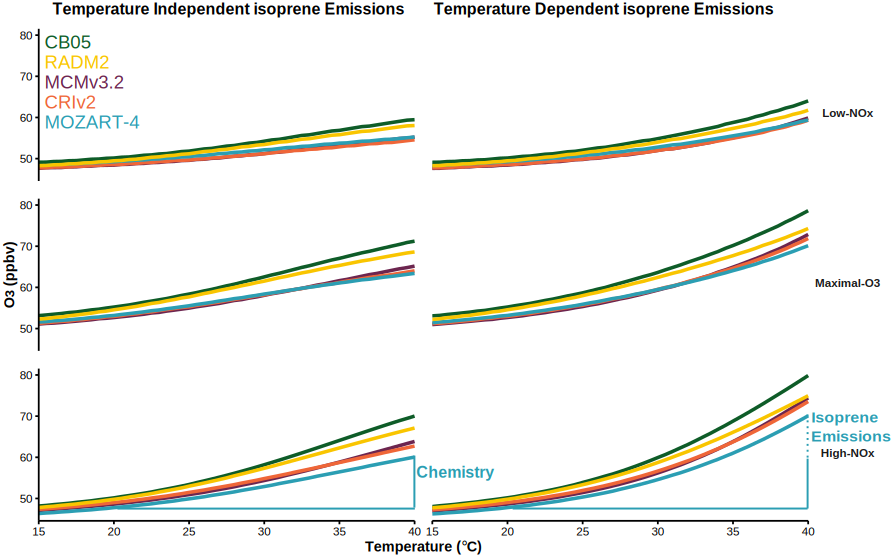
\includegraphics[width=\textwidth]{img/O3-T_correlation}%
\end{figure}

\begin{table}%
    \centering%
    \caption{Increase in ozone mixing ratio (ppbv) due to chemistry and emissions at $40$~\degree C from reference temperature ($20$~\degree C) in the \ce{NO_x}-regimes of Fig.~\ref{f:O3-T}.}%
    \label{t:differences}%
    \begin{tabularx}{\textwidth}{c|c *{3}{|c}} 
    \hline \hline
    \textbf{Chemical} & \textbf{Source of} & \multicolumn{3}{c}{\textbf{Increase in Ozone from 20~$^{\circ}$C to 40~$^{\circ}$C (ppbv)}} \\ \cline{3-5}
    \textbf{Mechanism} & \textbf{Difference} & \textbf{Low-\chem{NO_x}} & \textbf{Maximal-\chem{O_3}} & \textbf{High-\chem{NO_x}} \\ 
    \hline \hline
    \multirow{2}{*}{MCMv3.2} & Isoprene Emissions & 4.6 & 7.7 & 10.6 \\ 
    & Chemistry & 6.8 & 12.5 & 15.2 \\ \hline
    \multirow{2}{*}{CRIv2} & Isoprene Emissions & 4.8 & 7.9 & 10.8 \\
    & Chemistry & 6.0 & 11.1 & 13.7 \\ \hline
    \multirow{2}{*}{MOZART-4} & Isoprene Emissions & 4.1 & 6.7 & 10.0 \\
    & Chemistry & 6.0 & 10.2 & 12.3 \\ \hline
    \multirow{2}{*}{CB05} & Isoprene Emissions & 4.6 & 7.4 & 9.8 \\
    & Chemistry & 9.3 & 16.0 & 19.9 \\ \hline
    \multirow{2}{*}{RADM2} & Isoprene Emissions & 3.8 & 5.7 & 7.8 \\ 
    & Chemistry & 8.6 & 14.1 & 17.3 \\
    \hline \hline
\end{tabularx}
%
\end{table}

Figure~\ref{f:ozone_contours} depicts the maximum mixing ratio of ozone as a function of the total \ce{NO_x} emissions on the first day of simulations and temperature when using a temperature-independent and temperature-dependent source of isoprene emissions for each chemical mechanism.
A non-linear relationship of ozone mixing ratios with \ce{NO_x} and temperature is reproduced by each chemical mechanism.
This non-linear relationship is similar to that determined by \citet{Pusede:2014} using an analytical model constrained to observational measurements over the San Joaquin Valley in California.

Higher ozone mixing ratios are produced when using a temperature-dependent source of isoprene emissions (Fig.~\ref{f:ozone_contours}).
The highest mixing ratios of ozone are produced at high temperatures and moderate emissions of \ce{NO_x} regardless of the source of isoprene emissions.
Conversely, the least amount of ozone is produced with low emissions of \ce{NO_x} over the whole temperature range ($15$~--~$40$~\degree C) when using both a temperature-independent and temperature-dependent source of isoprene emissions.

The contours of ozone mixing ratios as a function of \ce{NO_x} and temperature can be split into three \ce{NO_x} regimes (Low-\ce{NO_x}, Maximal-\ce{O3} and High-\ce{NO_x}), similar to the \ce{NO_x} regimes defined for the non-linear relationship of ozone with VOC and \ce{NO_x}.
The Low-\ce{NO_x} regime corresponds with regions with little increase in ozone with temperature, also called the \ce{NO_x}-sensitive regime.
The High-\ce{NO_x} (or \ce{NO_x}-saturated) regime is when ozone levels increase rapidly with temperature and the contour ridges correspond to regions of maximal ozone production.
This is the Maximal-\ce{O3} regime.
\citet{Pusede:2014} showed that temperature can be used as a proxy for VOC, thus we assigned the ozone mixing ratios from each box model simulation to a \ce{NO_x} regime based on the ratio of \ce{HNO3} to \ce{H2O2}.
This ratio was used by \citet{Sillman:1995} to designate ozone to \ce{NO_x} regimes based on \ce{NO_x} and VOC levels.

Fig.~\ref{f:O3-T} illustrates the mean ozone mixing ratio at each temperature in the \ce{NO_x} regimes for each chemical mechanism and each type of isoprene emissions (temperature independent and temperature dependent).  
We define the absolute increase in ozone at $40$~\degree C from $20$~\degree C due to faster reaction rates as the difference between ozone mixing ratios at $40$~\degree C and $20$~\degree C when using a temperature-independent source of isoprene emissions.
When using a temperature-dependent source of isoprene emissions, the difference in ozone mixing ratios at $40$~\degree C from $20$~\degree C minus the increase due to faster chemistry, gives the absolute increase in ozone due to increased isoprene emissions.
These differences are represented graphically in Fig.~\ref{f:O3-T} and summarised in Table~\ref{t:differences}.

Table~\ref{t:differences} shows that the absolute increase in ozone with temperature due to faster chemistry is larger than the absolute increase in ozone due to increased isoprene emissions for each chemical mechanism and each \ce{NO_x} regime.
In all cases the absolute increase in ozone is largest under High-\ce{NO_x} conditions and lowest with Low-\ce{NO_x} conditions (Fig.~\ref{f:O3-T} and Table~\ref{t:differences}).
The increase in ozone mixing ratio at $40$~\degree C from $20$~\degree C due to faster chemistry with High-\ce{NO_x} conditions is almost double that under Low-\ce{NO_x} conditions.

In the Low-\ce{NO_x} regime, the increase of ozone with temperature using the reduced chemical mechanisms (CRIv2, MOZART-4, CB05 and RADM2) is similar to that from the MCMv3.2, larger differences occur in the Maximal-\ce{O3} and High-\ce{NO_x} regimes.
All reduced chemical mechanisms except RADM2 have similar increases in ozone due to increased isoprene emissions to MCMv3.2 (Table~\ref{t:differences}).
RADM2 produces $3$~ppbv less ozone than the MCMv3.2 due to increased isoprene emissions in each \ce{NO_x} regime, indicating that this difference is due the representation of isoprene degradation chemistry in RADM2.
These differences between the chemical mechanisms shall be explored in Sect.~\ref{ss:r_budgets}.

The Tagged Ozone Production Potential (TOPP) defined in \citet{Butler:2011} is a measure of the number of molecules of ozone produced per molecule of VOC emitted.
\citet{Coates:2015} compared ozone production in different chemical mechanisms to the MCMv3.2 using TOPPs and showed that less ozone is produced per molecule of isoprene emitted using RADM2 than with MCMv3.2.
The degradation of isoprene has been extensively studied and it is well-known that methyl vinyl ketone (MVK) and methacrolein are signatures of isoprene degradation \citep{Atkinson:2000}.
All chemical mechanisms in our study except RADM2 explicitly represent MVK and methacrolein (or in the case of CB05, a lumped species representing both these secondary degradation products).
RADM2 does not represent methacrolein and the mechanism species representing ketones (KET) is a mixture of acetone and methyl ethyl ketone (MEK) \citep{Stockwell:1990}. 
Thus the secondary degradation of isoprene in RADM2 is unable to represent the ozone production from the further degradation of the signature secondary degradation products of isoprene, MVK and methacrolein.
Updated versions of RADM2, RACM \citep{Stockwell:1997} and RACM2 \citep{Goliff:2013}, sequentially included methacrolein and MVK and with these updates the TOPP value of isoprene approached that of the MCMv3.2 \citep{Coates:2015}.

\subsection{Ozone Production Budgets} \label{ss:r_budgets}

\begin{figure}[t]%
    \centering%
    \caption{Day-time \ce{O_x} production budgets normalised by the total oxidation rate of emitted VOC in the \ce{NO_x}-regimes of Fig.~\ref{f:O3-T}. The budgets are allocated to categories of inorganic reactions, peroxy nitrate (RO2NO2) decomposition, reactions of NO with HO2, alkyl peroxy radicals (RO2) and acyl peroxy radicals (ARO2). All other reactions contributing to \ce{O_x} budgets are allocated to the `Other Organic' category.}%
    \label{f:ozone_budgets}%
    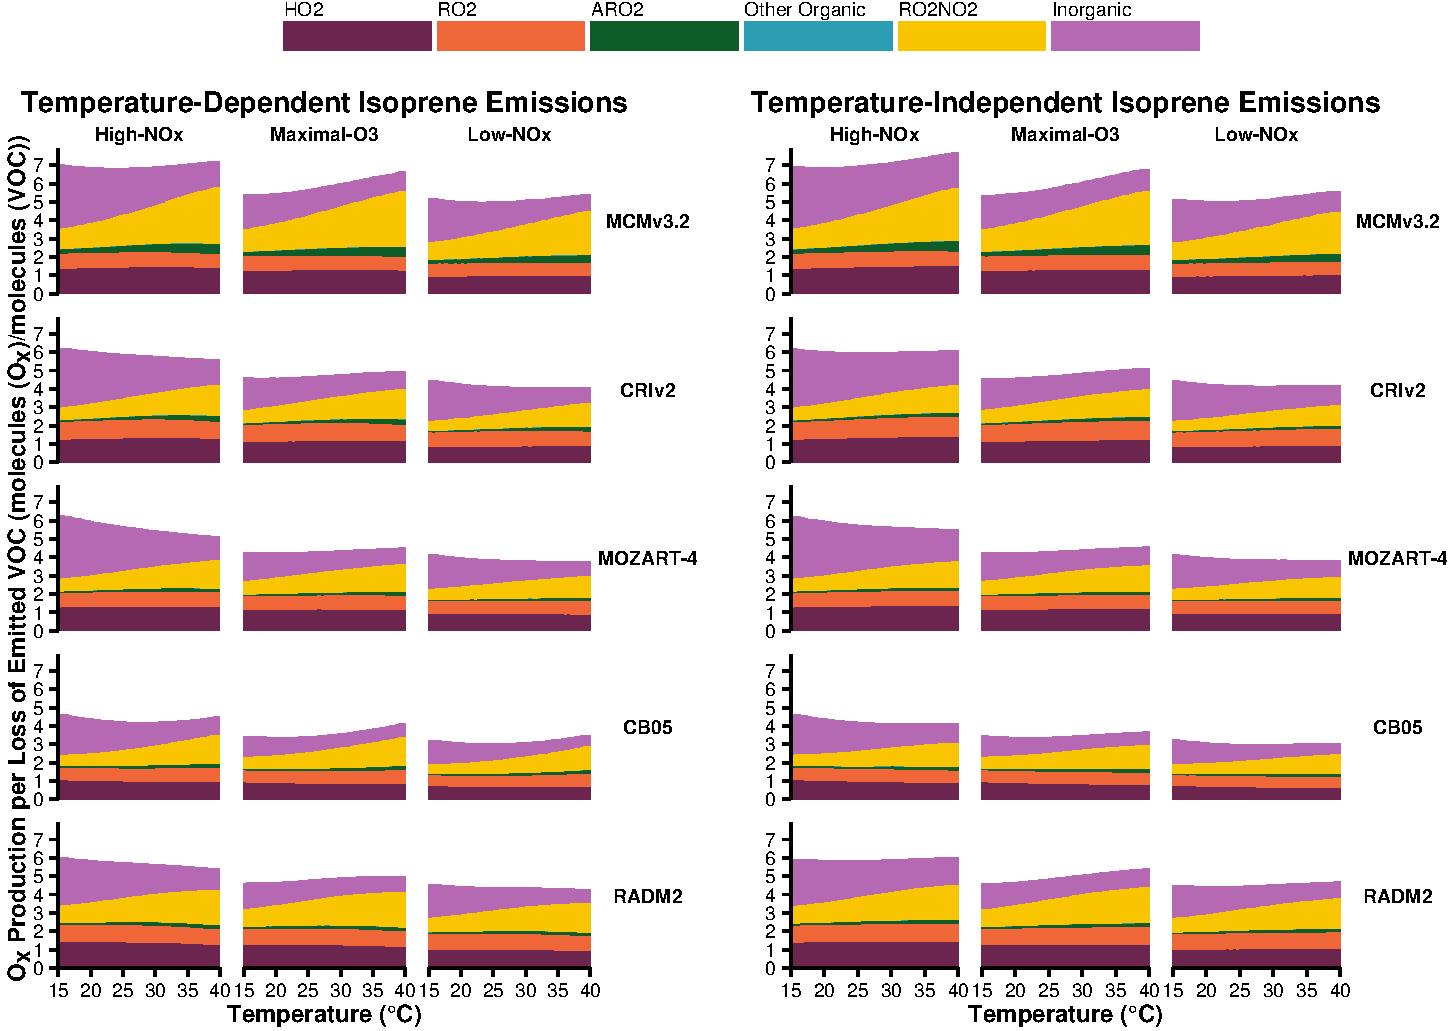
\includegraphics[width=\textwidth]{img/Ox_budgets}
\end{figure}

The total day-time production budgets of \ce{O_x} ($\equiv$ \ce{O3 + NO2 + O}) normalised by the total rate of oxidation of the emitted VOC are displayed in Fig.~\ref{f:ozone_budgets}.
The \ce{O_x} production budgets are assigned to each \ce{NO_x} regime for each chemical mechanism and source of isoprene emissions.
The budgets are allocated to the major sources, where `HO2', `RO2', `ARO2' represent the reactions of NO with \ce{HO2}, alkyl peroxy radicals and acyl peroxy radicals respectively.
`RO2NO2' represents the thermal decomposition of peroxy nitrates, `Inorganic' represents all inorganic contributions to \ce{O_x} production (primarily the de-excitation of \ce{O^1D} to O) and any other remaining organic reactions producing \ce{O_x} are included in the `Other Organic' category.

In Fig.~\ref{f:ozone_budgets}, a similar number of molecules of \ce{O_x} per molecule of emitted VOC oxidised are produced in High-\ce{NO_x} conditions when using either temperature-dependent or temperature-independent isoprene emissions for each chemical mechanism, the same occurs for the Maximal-\ce{O3} and Low-\ce{NO_x} regimes.
Thus the increases in ozone production due to increased emissions of isoprene with temperature are balanced by the faster oxidation rates at higher temperatures.
The largest amount of \ce{O_x} is produced in the High-\ce{NO_x} regime and the lowest amount of \ce{O_x} is produced in the Low-\ce{NO_x} regime, mirroring the \ce{O3} mixing ratios in the different \ce{NO_x} regimes in Fig.~\ref{f:O3-T}.
For example, MCMv3.2 produces seven molecules of \ce{O_x} per molecule of emitted VOC oxidised in High-\ce{NO_x} conditions decreasing to about six and five molecules of \ce{O_x} per molecule of emitted VOC oxidised in the Maximal-\ce{O3} and Low-\ce{NO_x} regimes.

Thermal decomposition of RO2NO2 contributes the most to the normalised \ce{O_x} production at higher temperatures in Fig.~\ref{f:ozone_budgets}, this contribution shows a strong dependency on temperature and is analysed further in Sect.~\ref{sss:ro2no2}.
The contributions of the reaction of NO with peroxy radicals (HO2, RO2 and ARO2 in Fig.~\ref{f:ozone_budgets}) to the normalised production of \ce{O_x} do not increase strongly with temperature indicating that the faster oxidation of emitted VOC at higher temperatures produces more peroxy radicals which when reacting NO fuels \ce{O_x} production.

The reduced chemical mechanisms produce up to two molecules of \ce{O_x} per molecule of emitted VOC oxidised less than the MCMv3.2 in each \ce{NO_x} regime despite the reduced chemical mechanisms producing similar absolute amounts of ozone to the MCMv3.2 (Fig.~\ref{f:ozone_contours} and Fig.~\ref{f:O3-T}).
At high temperatures, up to $86$~\% of the total difference in the normalised \ce{O_x} production using the reduced chemical mechanisms from the MCMv3.2 is due to differences in the contribution from peroxy nitrate (RO2NO2) decomposition.
These differences shall be explored in more detail in Sect.~\ref{sss:ro2no2}.

\subsubsection{Peroxy Nitrates} \label{sss:ro2no2}
Peroxy nitrates are formed from the reactions of peroxy radicals (\ce{RO2}) with \ce{NO2} (\ref{r:RO2_NO2}) and are an important reservoir species for both peroxy radicals and \ce{NO_x}.
\begin{rxnarray}
    && \ce{RO2 + NO2 + M} \rightleftharpoons \ce{RO2NO2 + M} \label{r:RO2_NO2}
\end{rxnarray}
The chemical bond of \ce{RO2NO2} is relatively weak and thermal decomposition is the most important chemical process with the rate of thermal decomposition increasing strongly with temperature.
At low temperatures, \ce{RO2NO2} can accumulate and be transported downwind of the emissions of the sources of its precursors (VOC and \ce{NO_x}) and after thermal decomposition the release of \ce{NO2} and peroxy radicals can promote production of \ce{O3} in regions devoid of large \ce{NO_x} sources \citep{Moxim:1996}.

Peroxy nitrates are formed from both alkyl and acyl peroxy radicals produced during the secondary degradation of emitted VOC.
The most important alkyl peroxy nitrates are pernitric acid (\ce{HO2NO2}) and methylperoxy nitrate (\ce{CH3O2NO2}), while peroxy acetyl nitrate (PAN, \ce{CH3C(O)O2NO2}) and peroxy propionyl nitrate (PPN, \ce{C2H5C(O)O2NO2}) are important acyl peroxy nitrates.
The alkyl peroxy nitrates have a weaker \ce{RO2-NO2} bond than acyl peroxy nitrates hence alkyl peroxy nitrates have a shorter lifetime than acyl peroxy nitrates.
At $298$~K, the lifetime of \ce{CH3O2NO2} is $0.5$~seconds while PAN has a lifetime of $51$~minutes \citep{Orlando:2012}.

Each chemical mechanism used in our study represents \ce{HO2NO2} and PAN, although in many reduced chemical mechanisms the PAN mechanism species represents \ce{CH3C(O)O2NO2} and other acyl peroxy nitrates.
This representation of PAN in reduced chemical mechanisms can overestimate PAN levels compared to more detailed chemical mechanisms \citep{Luecken:1999}.
The near-explicit MCMv3.2 represents a range of peroxy nitrates including \ce{CH3O2NO2} and about $280$~acyl peroxy nitrates.

\begin{figure}[t]%
    \centering%
    \caption{Day-time \ce{RO2NO2} production budgets normalised by the total oxidation rate of emitted VOC in the \ce{NO_x}-regimes of Fig.~\ref{f:O3-T}. The total budgets are allocated to the most important peroxy nitrates and all other contributions included as `Others'.}%
    \label{f:ro2no2_budgets}%
    \includegraphics[width=\textwidth]{img/RO2NO2_budgets}
\end{figure}

Figure~\ref{f:ro2no2_budgets} displays the normalised production budgets of \ce{RO2NO2} by the total oxidation rate of the emitted VOC for each chemical mechanism in each \ce{NO_x} regime with a temperature-independent and temperature-dependent source of isoprene emissions.
The contribution of \ce{CH3O2NO2} to normalised \ce{RO2NO2} production in MCMv3.2 is missing from the budgets of each reduced chemical mechanism as \ce{CH3O2NO2} is not represented in any of the reduced chemical mechanisms.
In fact when removing the contribution of \ce{CH3O2NO2} to normalised \ce{RO2NO2} production in MCMv3.2, the normalised \ce{RO2NO2} production of the reduced chemical mechanisms is similar to that in the MCMv3.2 for each \ce{NO_x} regime and regardless of isoprene source.
Including \ce{CH3O2NO2} chemistry in reduced chemical mechanisms would improve the representation of the total \ce{RO2NO2} production having the added benefit of improving the representation of \ce{O_x} production budgets in Fig.~\ref{f:ozone_budgets}.

\subsection{Comparison to Observations and 3D Model Simulations} \label{ss:r_observations}
 \begin{figure}%
    \centering%
    \caption{The maximum 8~h mean ozone from the box model simulations allocated to the different \ce{NO_x} regimes for each chemical mechanisms (solid lines). The box model ozone-temperature correlation is compared to the summer 2007 ERA-Interim data (black circles) and WRF-Chem output using MOZART-4 (purple boxes) and RADM2 (orange triangles).}%
    \label{f:comparison}%
    \begin{subfigure}[t]{\textwidth}%
        \centering%
        \vspace{2mm}%
        \caption{Ozone-Temperature correlation over central and eastern Germany}%
        \label{f:WRF_ERA_Germany}%
        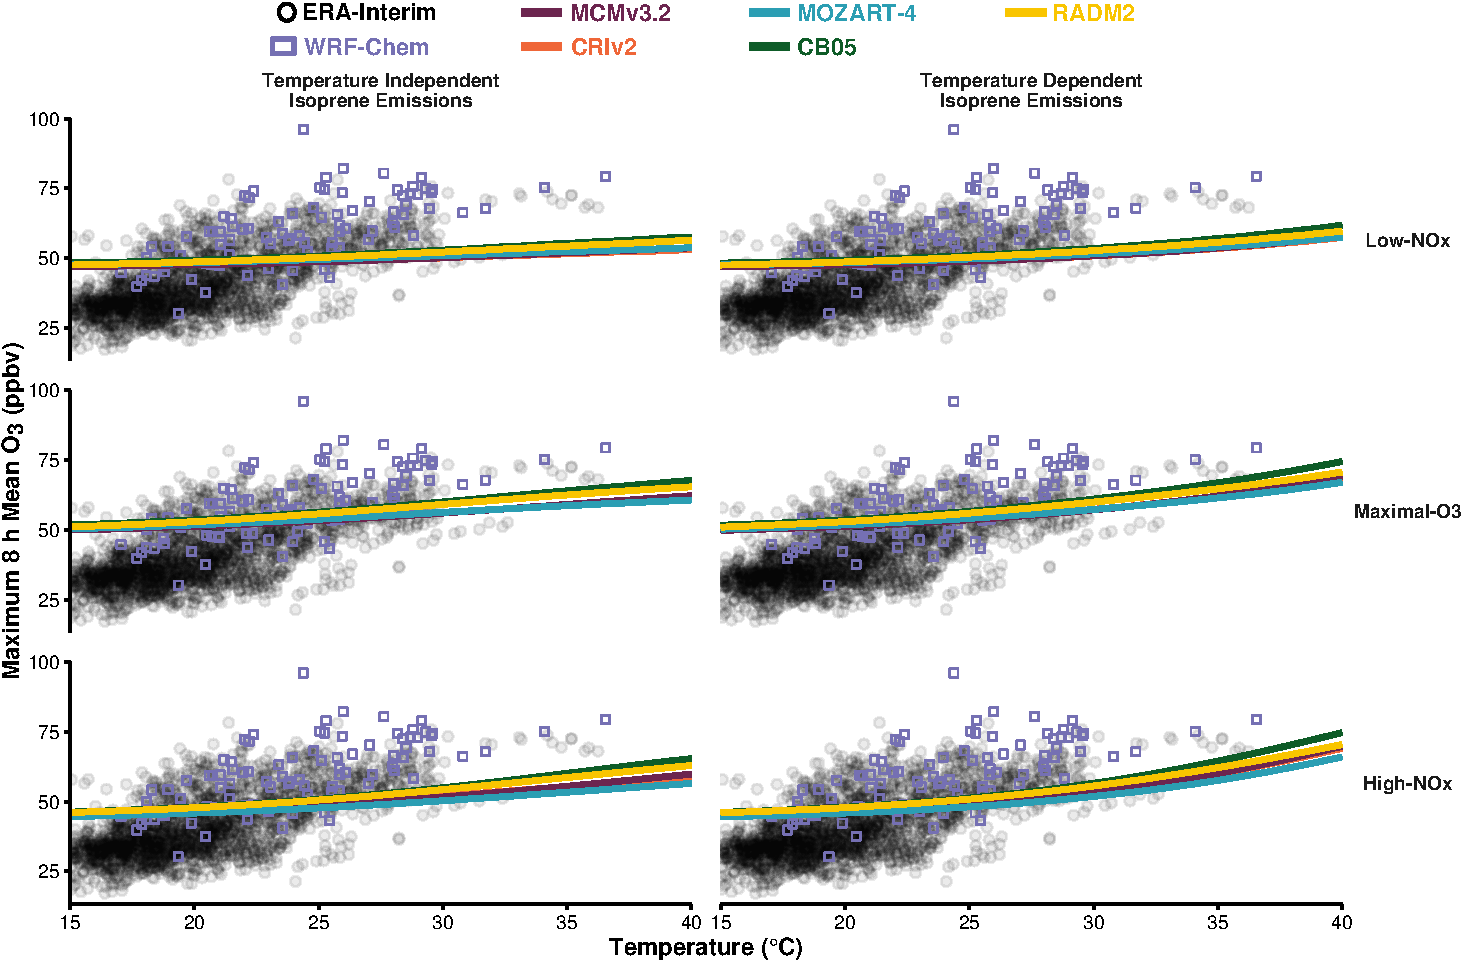
\includegraphics[height=0.43\textheight]{img/Germany_O3-T_ERA_WRF_2007}%
    \end{subfigure}%
    \\
    \begin{subfigure}[t]{\textwidth}%
        \caption{Ozone-Temperature correlation over central and western Poland}%
        \label{f:WRF_ERA_Poland}%
        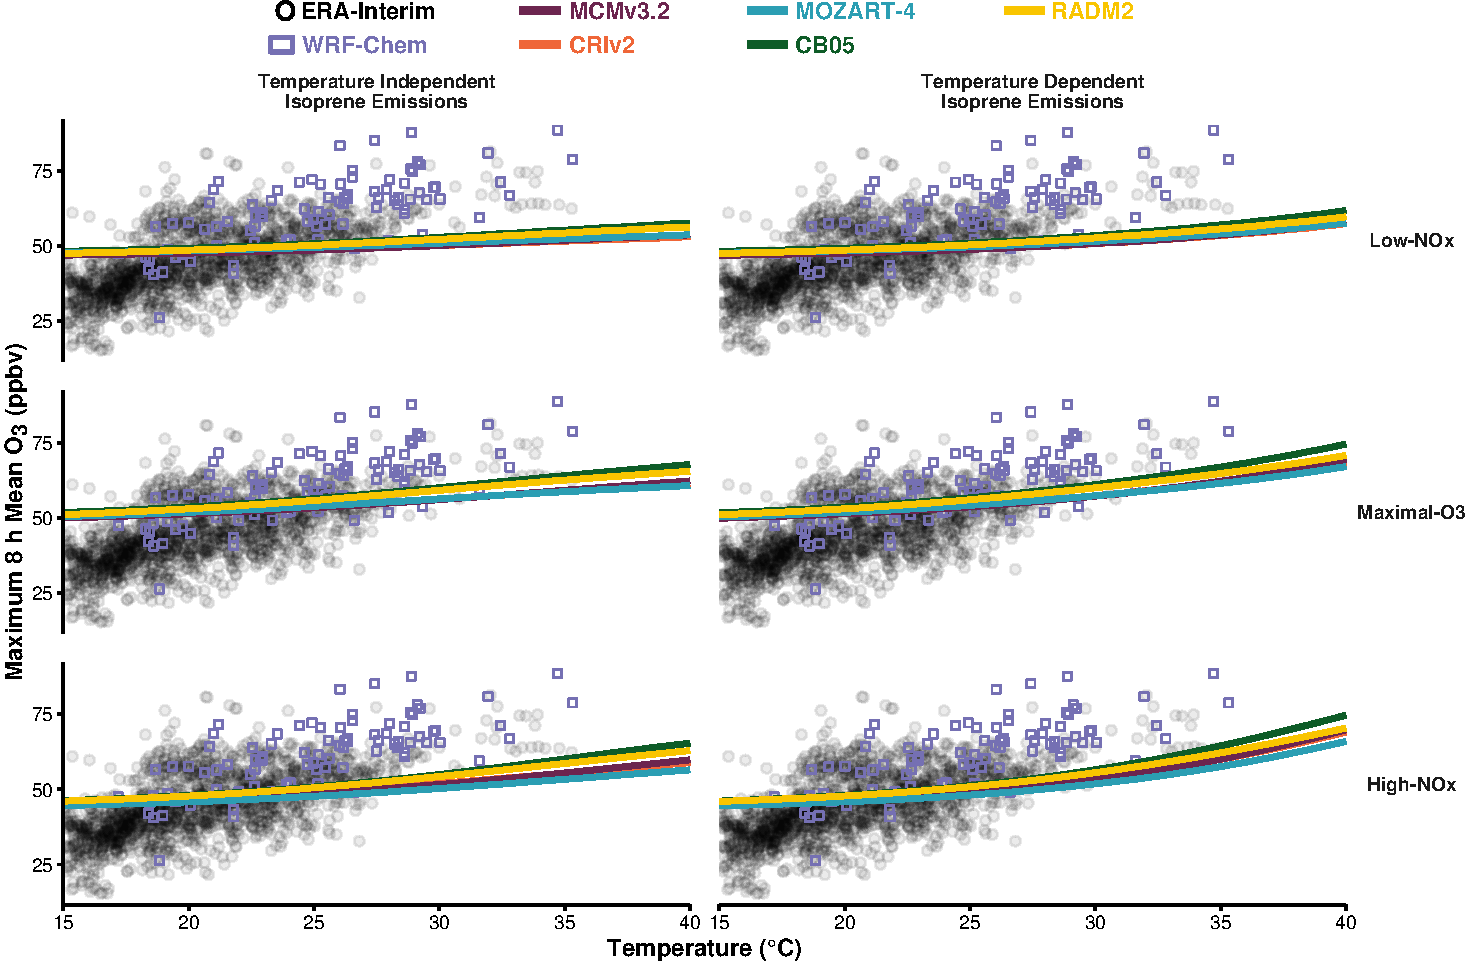
\includegraphics[height=0.43\textheight]{img/Poland_O3-T_ERA_WRF_2007}%
    \end{subfigure}%
\end{figure}

\begin{table}[t]%
    \centering%
    \caption{Slopes (m$_{\text{O3-T}}$ in ppbv per \degree C) of the linear fit to the ozone-temperature correlations in Fig.~\ref{f:comparison}}%
    \label{t:mo3-t}%
    \begin{subtable}[t]{\textwidth}%
        \centering%
        \vspace{2mm}%
        \caption{Slope of linear fit of the ERA-Interim observational data and WRF-Chem model output using MOZART-4 and RADM2 chemistry over central and eastern Germany and western and central Poland.}%
        \label{t:era_wrf_o3-T}%
        {\renewcommand{\arraystretch}{1.2}
\begin{tabular}{r|c|c}
	\hline\hline
    & \textbf{Germany} & \textbf{Poland} \\
	\hline\hline
	 ERA-Interim & 2.15 & 1.94 \\
	 WRF-Chem with MOZART-4 & 2.05 & 2.00 \\
	 WRF-Chem with RADM2 & 1.78 & 1.77 \\
	\hline\hline
\end{tabular}}
%
    \end{subtable}
    \begin{subtable}[t]{\textwidth}%
        \centering%
        \vspace{2mm}
        \caption{Slope of linear fit of box model experiments for each chemical mechanism, source of isoprene emissions allocated to the three \ce{NO_x}-regimes.}%
        \label{t:boxmodel_o3-T}%
        \scalebox{.78}[.78]{{\renewcommand{\arraystretch}{1.2}
\begin{tabular}{c|c|cc|cc|cc}
	\hline\hline
    \multirow{2}{*}{\textbf{Mechanism}} & \multirow{2}{*}{\textbf{Isoprene Emissions}} & \multicolumn{2}{c|}{\textbf{Low-\chem{NO_x}}} & \multicolumn{2}{c}{\textbf{Maximal-\chem{O_3}}} & \multicolumn{2}{|c}{\textbf{High-\chem{NO_x}}} \\
    & & \textbf{Mixing} & \textbf{No Mixing} & \textbf{Mixing} & \textbf{No Mixing} & \textbf{Mixing} & \textbf{No Mixing} \\
	\hline\hline
	\multirow{2}{*}{MCMv3.2} & Temperature Independent & 0.28 & 1.01 & 0.51 & 1.36 & 0.59 & 0.96 \\ 
    & Temperature Dependent & 0.42 & 1.48 & 0.74 & 2.16 & 0.93 & 2.63 \\ 
	\hline
	\multirow{2}{*}{CRIv2} & Temperature Independent & 0.25 & 0.93 & 0.47 & 1.27 & 0.55 & 0.88 \\ 
    & Temperature Dependent & 0.40 & 1.44 & 0.71 & 2.09 & 0.90 & 2.52 \\ 
	\hline
	\multirow{2}{*}{MOZART-4} & Temperature Independent & 0.25 & 0.97 & 0.44 & 1.21 & 0.49 & 0.59 \\ 
    & Temperature Dependent & 0.38 & 1.43 & 0.65 & 1.98 & 0.81 & 2.05 \\ 
	\hline
	\multirow{2}{*}{CB05} & Temperature Independent & 0.39 & 1.30 & 0.67 & 1.72 & 0.79 & 1.45 \\ 
    & Temperature Dependent & 0.52 & 1.72 & 0.89 & 2.44 & 1.12 & 2.94 \\ 
	\hline
	\multirow{2}{*}{RADM2} & Temperature Independent & 0.37 & 1.31 & 0.61 & 1.64 & 0.70 & 1.28 \\ 
    & Temperature Dependent & 0.48 & 1.68 & 0.79 & 2.22 & 0.97 & 2.49 \\ 
	\hline\hline
\end{tabular}}}
%
    \end{subtable}
\end{table} 

This section compares the results from our idealised box model simulations to real-world observations and model output from a 3D model.
\citet{Otero:2016} showed that over the summer (JJA) months, temperature is the main meteorological driver of ozone production over many regions of central Europe using the observational data set of the ERA-Interim re-analysis.
This data set includes the daily maximum temperature and daily maximum 8~h mean of ozone for the years 1998--2012 over Europe.
Model output from the 3D WRF-Chem regional model set-up over the European domain for simulations of the year 2007 using MOZART-4 and RADM2 chemistry from \citet{Mar:2016} was used to further compare the box model simulations to a model including more meteorological processes than the box model.

Figure~\ref{f:comparison} compares the observational (ERA-Interim) and WRF-Chem data from summer 2007 to the maximum 8~h mean ozone from the box model simulations for each chemical mechanism, \ce{NO_x} regime and type of isoprene emissions.
In Fig.~\ref{f:comparison}, we limited the observational data to days where the observed daily maximum temperature corresponded to the temperature range in our study ($15$--$40$~\degree C).
We selected two regions from the observations and WRF-Chem output, central and eastern Germany (Fig.~\ref{f:WRF_ERA_Germany}) and central and western Poland (Fig.~\ref{f:WRF_ERA_Poland}), where the summertime ozone values are driven by with temperature \citep{Otero:2016}.
Table~\ref{t:mo3-t} summarises the slopes (m$_{\text{O3-T}}$) of the linear fits of all the ozone-temperature correlations displayed in Fig.~\ref{f:comparison} in ppbv of ozone per \degree C determining the rate of change of ozone with temperature.

The spread of the observed ozone-temperature values over both Germany and Poland are generally captured by the combined WRF-Chem simulations with both MOZART-4 and RADM2 chemistry. 
However, the ozone-temperature data from WRF-Chem using MOZART-4 chemistry reproduces the higher ozone values with temperature from ERA-Interim but not the lower values.
On the other hand, WRF-Chem with RADM2 only reproduces the lower ozone values of the ERA-Interim data.
The differences between the ozone produced using WRF-Chem with MOZART-4 and RADM2 shall be addressed in \citet{Mar:2016}.
The rate of change of ozone with temperature from the WRF-Chem simulations using both MOZART-4 and RADM2 is similar to the rate of change of ozone with temperature from the observed data (Table~\ref{t:era_wrf_o3-T}).

The differences in ozone production between the different chemical mechanisms with the box model are small compared to the spread of the ERA-Interim and WRF-Chem data.
When using a temperature-dependent source of isoprene emissions in the box model, the rate of change of ozone with temperature in the box model approaches that of the observed data, although still less than half that of the observations.
The box model simulations using a temperature-independent source of isoprene emissions do not reproduce the range of observed ozone-temperature values (Table~\ref{t:mo3-t}).

A temperature-dependent source of isoprene with high-\ce{NO_x} conditions produces the most similar ozone-temperature slope to the observational data but this is still lower than the observed ozone-temperature slope by a factor of two.
In particular, the box model simulations over-predict the ozone values at lower temperatures and under-predict the ozone values at higher temperatures compared to the observed data.
Similarly, the rate of change of ozone with temperature in the box model is less-sensitive than WRF-Chem using MOZART-4 or RADM2 chemistry.

The main reason for the box model simulations being less sensitive to temperature than the observations and WRF-Chem simulations is related to the set-up of the box model.
Observations and the WRF-Chem simulations consider both the direct and indirect effects of temperature on ozone, while our box model only considered two direct effects of temperature on ozone.
Furthermore, observational studies represent at the total derivative of ozone with temperature while models consider the partial derivatives of the temperature-dependent processes influencing ozone \citep{Rasmussen:2013}. 
\begin{equation*} 
    \frac{d[\ce{O3}]}{dT} = \frac{\partial [\ce{O3}]}{\partial [\text{BVOC}]}\frac{\partial [\text{BVOC}]}{\partial T} + \frac{\partial [\ce{O3}]}{\partial \text{Chemistry}}\frac{\partial \text{Chemistry}}{\partial T} + \frac{\partial [\ce{O3}]}{\partial \text{Stagnation}}\frac{\partial \text{Stagnation}}{\partial T} + \dots
\end{equation*}

In our simulations, we focused on instantaneous production of ozone from a freshly-emitted source of VOC not considering stagnant atmospheric conditions.
In these atmospheric conditions, where high temperatures are present for multi-day periods, the ozone from the previous day is not transported away from the region leading to increased ozone levels when including the production of fresh ozone from new emissions.  
\citet{Otero:2016} showed that the previous day's ozone was also an important driver for observed ozone production over Europe.
3D models such as WRF-Chem that can simulate more realistic atmospheric conditions would play a valuable role for future work evaluating the ozone-temperature relationship at different \ce{NO_x} conditions at a regional scale.
